\documentclass[11pt,a4paper]{report} 
% Alternativ für doppelseitigen Ausdruck (nur bei > 60 Seiten sinnvoll)
%\documentclass[11pt,a4paper,twoside,openright]{report} 

% Deutsch
\usepackage[german]{babel} % deutsch und deutsche Rechtschreibung
\usepackage[utf8]{inputenc} % Unicode Text 
\usepackage[T1]{fontenc} % Umlaute und deutsches Trennen
\usepackage{textcomp} % Euro
\usepackage[hyphens]{url}
% statt immer Ab\-schluss\-ar\-beit zu schreiben
% einfach hier sammeln mit -. 
\hyphenation{Ab-schluss-ar-beit}
% Vorsicht bei Umlauten und Bindestrichen
\hyphenation{Ver-st\"ar-ker-aus-gang}
 % eigene Hyphenations, die für das Dokument gelten
\usepackage{amssymb} % Symbole
\usepackage{enumitem}
\usepackage{tabularx}


%% Fonts, ein kompletter Satz an Optionen
% Times New Roman, gewohnter Font mit ok tt und serifenlos
%\usepackage{mathptmx} 
%\usepackage[scaled=.95]{helvet}
%\usepackage{courier}
% Palatino, mal was anderes, auch mit ok tt und serifenlos
% empfohlen
\usepackage{mathpazo} % Palatino, mal was anderes
\usepackage[scaled=.95]{helvet}
\usepackage{courier}
% New Century Schoolbook sieht auch nett aus (macht auch tt und serifenlos)
%\usepackage{newcent}

% zusätzlich: Default serifenlos mit Helvetica 
% ich kann es nicht mehr sehen...
%\renewcommand{\familydefault}{\sfdefault}

\usepackage{microtype}

% Bilder und Listings
\usepackage{graphicx} % wir wollen Bilder einfügen
\usepackage{subfig} % Teilbilder
\usepackage{wrapfig} % vielleicht doch besser vermeiden
\usepackage{listings} % schöne Quellcode-Listings
% ein paar Einstellungen für akzeptable Listings
\lstset{basicstyle=\sffamily, columns=[l]flexible, mathescape=true, showstringspaces=false, numbers=left, numberstyle=\tiny}
\lstset{language=python} % und nur schöne Programmiersprachen ;-)
% und eine eigene Umgebung für Listings
\usepackage{float}
\newfloat{listing}{htbp}{scl}[chapter]
\floatname{listing}{Listing}

% Seitenlayout
%\usepackage[paper=a4paper,width=14cm,left=35mm,height=22cm]{geometry}
\usepackage[paper=a4paper,width=14cm,height=22cm]{geometry}
\usepackage{setspace}
\linespread{1.15}
\setlength{\parskip}{0.5em}
\setlength{\parindent}{0em} % im Deutschen Einrückung nicht üblich, leider

% Seitenmarkierungen 
\newcommand{\phv}{\fontfamily{phv}\fontseries{m}\fontsize{9}{11}\selectfont}
\usepackage{fancyhdr} % Schickere Header und Footer

\pagestyle{fancy}
\renewcommand{\chaptermark}[1]{\markboth{#1}{}}
\renewcommand{\sectionmark}[1]{\markright{#1}}
\fancyhead[LO]{\phv \nouppercase{\leftmark}}
\fancyhead[RE]{\phv \nouppercase{\rightmark}}
\fancyhead[RO,LE]{\phv \thepage}
\fancyfoot[C]{\ } % Seitenzahl unten nur Kapitel


% Theorem-Umgebungen
\newtheorem{definition}{Definition}[chapter]
\newtheorem{satz}{Satz}[chapter]
\newtheorem{lemma}[satz]{Lemma} % gleicher Zähler wie Satz
\newtheorem{theorem}{Theorem}[chapter]
\newenvironment{beweis}[1][Beweis]{\begin{trivlist}
\item[\hskip \labelsep {\textit{#1 }}]}{\end{trivlist}}
\newcommand{\qed}{\hfill \ensuremath{\square}}

% Inhaltsverzeichnis
\setcounter{tocdepth}{1}
\setcounter{secnumdepth}{2}

% Quellen teilen
\usepackage{bibtopic} 

% Hochschule Logo, noch nicht perfekt
\usepackage{hsrmlogo}

% Spezialpakete
\usepackage{epigraph}
\setlength{\epigraphrule}{0pt} % kein Trennstrich

% damit wir nicht so viel tippen müssen, nur für Demo 
\usepackage{blindtext} 

% Zum Zeigen von Fehlern
\usepackage{soul}
\newcommand*\falsch{\st}

% Links im PDF
\usepackage{hyperref}
\hypersetup{
    colorlinks=true,
    citecolor=black,
    filecolor=black,
    linkcolor=black,
    urlcolor=black
}

% Kommentare
\usepackage{comment} % alle Pakete und Einstellungen	
\usepackage{hyperref}
% Hier anpassen 
\newcommand{\titel}{Entwurf, prototypische Implementierung und Evaluation eines Sicherheitskonzepts für die Authentifizierung und Autorisierung von Fernzugriffen auf eine Automatisierungsanlage}
\newcommand{\kurztitel}{Template Abschlussarbeit}
\newcommand{\autor}{Kevin Sapper}
\newcommand{\datum}{09. Oktober 2014} % Abgabedatum
\newcommand{\ort}{Wiesbaden}
\newcommand{\referent}{Prof.\ Dr.\ Reinhold Kröger}
\newcommand{\korreferent}{Prof.\ Dr.\ Martin Gergeleit}

\begin{document}
\pagenumbering{Roman}

\begin{titlepage}
  \begin{center}
    % Kopf der Seite
    \hsrmlogo[1]
    \parbox[b]{8cm}{Hochschule RheinMain \\
     Fachbereich Design Informatik Medien \\
     Studiengang Angewandte Informatik}
    \vfill    
    {\LARGE Abschlussarbeit} \\[0.5cm]
    {\large zur Erlangung des akademischen Grades} \\[5mm]
    {\large Bachelor of Science (B.Sc.)} \\[5mm]
    \rule{\textwidth}{1pt}\\[0.5cm]
    {\begin{spacing}{1.15} \huge \bfseries \titel \\ \end{spacing}}
    \rule{\textwidth}{1pt}    
    \vfill    
    \begin{tabular}{ll} % Mitte der Seite
      Vorgelegt von & \autor \\
      am & \datum \\
      Referent & \referent \\
      Korreferent & \korreferent
    \end{tabular}    
    \vfill
  \end{center}
\end{titlepage}
\cleardoublepage


% Erklärung gemäß den Allgemeinen Bestimmungen für Prüfungsordnungen
% der Paragraph schwankt, daher ohne Nennung einer Nummer
\section*{Erklärung gemäß ABPO}
\thispagestyle{empty}
Ich erkläre hiermit,
\begin{itemize}
\item dass ich die vorliegende Abschlussarbeit selbstständig angefertigt,
\item keine anderen als die angegebenen Quellen benutzt,
\item die wörtlich oder dem Inhalt nach aus fremden Arbeiten entnommenen 
  Stellen, bildlichen Darstellungen und dergleichen als solche genau 
  kenntlich gemacht und
\item keine unerlaubte fremde Hilfe in Anspruch genommen habe.
\end{itemize}

\vspace{6em}
\noindent\begin{tabular}{p{0.37\textwidth}p{0.56\textwidth}}
\ort, \datum  & \rule{0.56\textwidth}{0.5pt}\\
              & \makebox[1cm]{\ } \autor
\end{tabular}

\vfill

\section*{Erklärung zur Verwendung der Bachelor Thesis}

Hiermit erkläre ich mein Einverständnis mit den im folgenden 
aufgeführten Verbreitungsformen dieser Abschlussarbeit:

\vspace{1em}
\noindent\begin{tabular}{|p{0.82\textwidth}|c|c|}
  \hline
  \textbf{Verbreitungsform} & \makebox[0.035\textwidth]{\textbf{Ja}} 
                            & \makebox[0.05\textwidth]{\textbf{Nein}} \\\hline
  Einstellung der Arbeit in die Hochschulbibliothek 
                         mit Datenträger   &  & $\times$ \\\hline
  Einstellung der Arbeit in die Hochschulbibliothek  
                         ohne Datenträger  & $\times$ & \\\hline
  Veröffentlichung des Titels der Arbeit im Internet  
                                           & $\times$ & \\\hline
  Veröffentlichung der Arbeit im Internet             
                                           & $\times$ & \\\hline
\end{tabular}

\vspace{6em}
\noindent\begin{tabular}{p{0.37\textwidth}p{0.56\textwidth}}
\ort, \datum  & \rule{0.56\textwidth}{0.5pt}\\
              & \makebox[1cm]{\ } \autor
\end{tabular}
\cleardoublepage

 % Titelseite, Erklärungen, etc.

\begin{comment}
\begin{abstract} 
\LaTeX\ bietet Buchdruckqualität für jedermann.
Wir zeigen anhand dieses durch persönliche Präferenzen geprägtes Template, 
wie man Buchdruckqualität für eine Abschlussarbeit einfach erreichen kann.
Dazu sind beispielhaft Lösungen zu üblichen Fragestellungen im Dokument 
demonstriert.
Neben den grundlegenden For\-ma\-tie\-rungs\-möglich\-keiten mit \LaTeX\ wird 
insbesondere das Erstellen und Einbinden von Grafiken und Listings gezeigt.
Des Weiteren werden Literatur- und andere Verzeichnisse eingebunden.
Nicht zuletzt finden sich auch sachdienliche Hinweise zum
Schreiben.
\end{abstract}

\epigraphhead[70]{\epigraph{The user's going to pick dancing pigs over security every time.}{\textit{Bruce Schneier}}}
\epigraphhead[70]{\epigraph{Companies spend millions of dollars on firewalls, encryption and secure access devices, and it’s money wasted, because none of these measures address the weakest link in the security chain.}{\textit{Kevin Mitnick}}}
\epigraphhead[70]{\epigraph{Wisdom consists in being able to distinguish among dangers and make a choice of the least harmful.}{\textit{Niccolo Machiavelli, The Prince}}}
\epigraphhead[70]{\epigraph{Using encryption on the Internet is the equivalent of arranging an armored car to deliver credit card information from someone living in a cardboard box to someone living on a park bench.}{\textit{Gene Spafford}}}
\end{comment}

\tableofcontents
\clearpage 

\pagenumbering{arabic}

\chapter{Einführung} \label{chap:intro}

\begin{itemize}
\item Entwurf -- CATWOE soft systems methodology (SSM)
\item Sicherheitskonzept
\item Authentifizerung \& Autorisierung
\item Fernzugriff
\item Automatisierungsanlage
\item Evaluation
\item prototypische Implementierung
\end{itemize}

\chapter{Problemfeld} \label{chap:problem}
 
Im Bereich Kältetechnik wird Regelungstechnik zur Vernetzung und Überwachung von Kälteanlagen entwickelt. Hierzu gehören die Produkte aus der E*LDS Reihe. Diese beinhalten Verbundsteuerungen zur Kälteerzeugung, Kühlstellenregler zur temperaturgenauen Reglung aller Arten von Kühlmöbeln und Kühlräumen, Funk-Temperatursensoren und der Marktrechner als zentrale Intelligenz einer Kälteanlage. Das Team Datentechnik entwickelt die Software für den Marktrechner und stellt das zu behandelnde Problemfeld. 

\section{Aktuelle Situation}

Der Marktrechner ist das Herzstück einer Kälteanlage. Über einen CAN-Bus ist er mit allen Komponenten der Anlage verbunden. Er ist in der Lage, Komponenten zentral zu parametrieren und zu überwachen. Auf dem internen Speicher werden sämtliche Betriebsdaten und Betriebszustände, Meldungen und Alarme archiviert. Die 24-Stunden Überwachung vor Ort durch einen Mitarbeiter ist bei der Menge an Anlagen nicht wirtschaftlich. Deshalb werden heutzutage Fernservice-Zentralen eingesetzt. Aktuell sind Fernservice-Zentralen über VPN mit einem oder mehreren Unternehmensnetzwerken, ihrer Kunden, verbunden. Über dieses können die Marktrechner erreicht werden. Auf diese Weise kann eine einzige Fernservice-Zentrale Tausende Marktrechner überwachen. Tritt ein Fehler auf, kann die Fernservice-Zentrale entweder direkt eingreifen oder einen Monteur zum betreffenden Kunden schicken, der die Anlage instand setzt.

\begin{comment}
@startuml

package "Unternehmensnetzwerk A" as UA {
  [Marktrechner 1]
  [Marktrechner 2]
  [...]
  [Marktrechner n]
}

package "Unternehmensnetzwerk B" as UB {
}

package "Unternehmensnetzwerk C" as UC {
}

cloud VPN {
}

["Fernservice-Zentrale"] -down- VPN
VPN -down- UA
VPN -left- UB
VPN -right- UC
UA - [Marktrechner n]
UA - [...]
UA - [Marktrechner 2]
UA - [Marktrechner 1]

@enduml
\end{comment}

\begin{figure}[h]
\centering
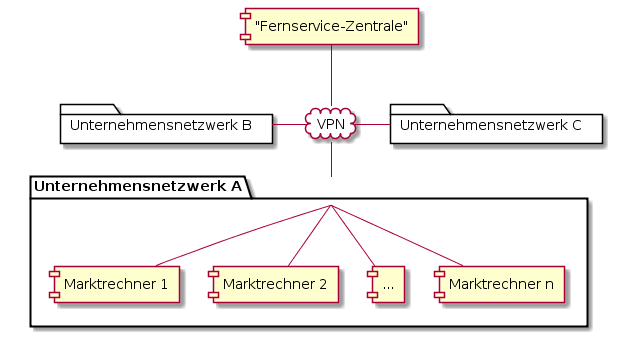
\includegraphics[scale=0.5]{thesis.png}
\caption{Aktuelle Vernetzung}
\label{fig:current_setup}
\end{figure}

Über VPN ist die Kommunikation von der Fernservice-Zentrale bis zum Unternehmensnetzwerk abgesichert. Im Netzwerk des Unternehmens ist der gesamte Datenverkehr zu und von den Marktrechnern allerdings unverschlüsselt. Daten könnten somit von jedem Teilnehmer im Netzwerk mitgelesen werden. Darüber hinaus wäre der Zugriff auf die Daten bei bekannter IP-Adresse möglich, denn es gibt keine geeignete Authentifizierung und Autorisierung. Insbesondere bei Aufrufen zur Systemveränderung kann dies zu Problemen führen. Der aktuelle Zugriff auf die Daten wird über Webservices, auf Basis von einfachen XML-RPCs, realisiert. Im Rahmen des absolvierten Praktikums wurde eine neue Webservice-Schnittstelle geschrieben, welcher das weit verbreitete REST-Konzept für Webanwendungen zu Grunde liegt. Das RestGateway führt zur Zeit keine Authentifizierung und Autorisierung durch. Es wurde aber mit dem Hintergrund entwickelt, diese Funktionen zu integrieren.

\chapter{Bedrohungsmodell} \label{chap:threat}
\epigraphhead[70]{\epigraph{The only truly secure system is one that is powered off, cast in a block of concrete and sealed in a lead-lined room with armed guards.}{\textit{Gene Spafford}}}

Das Bedrohungsmodell soll auf mögliche Gefahren des aktuellen Systems hinweisen und diese schrittweise, durch geeignete Maßnahmen, eindämmen. Eine geeignete Analyse- und Designmethodik dazu bietet die Soft Systems Methodology (SSM). Besonderes Augenmerk findet die Trennung von realer und theoretischer Problemsituation. In der ersten Phase soll das gesamte Problemfeld aus Sicher aller beteiligten herausgefunden werden. Anschließend werden diese Informationen, der relevante Problembereich, theoretisch aus Sicht eines Verteidiger und eines Angreifers beschrieben und jeweils ein konzeptionelles Modell erstellt. Die Modelle werden zum Schluss gegeneinander und gegen die reale Welt verglichen. Dadurch soll eine möglichst große Abdeckung im Gefahrenpotential erreicht werden.

\section{Finding out}

\section{Defender} 

\subsection{Formulation of Root Definitions}

\subsection{Building Conceptual Model}

\subsection{Compare Model with Real World}

\section{Attacker}

\subsection{Formulation of Root Definitions}

\subsection{Building Conceptual Model}

\subsection{Compare Model with Real World}

\chapter{Entwurf oder Design} \label{chap:design}

\chapter{Evaluation} \label{chap:evaluation}


\chapter{Bilder und Listings} \label{chap:bilder}

Bilder werden meist unabhängig von \LaTeX\ erstellt und dann nur 
eingebunden. 
Bilder, genau wie Tabellen, Listings oder ähnliches, sind dabei nicht 
Teil des normalen Fließtexts sondern separate Objekte, 
deren Position sich nach Gutdünken des Setzers (also \LaTeX) 
ändern kann.
Diese fließenden Objekte, oder auch Fließobjekte,
beinhalten dann das Bild, das Listing oder die Tabelle.

\section{Fließobjekte}

Bilder, Listings und Tabellen sollten als Fließobjekte (\emph{floats}) 
oder Float-Objekte gesetzt werden.
Das heißt \LaTeX\ entscheidet wohin das Objekt kommt, man selbst
gibt nur Hinweise wo es gut wäre.
Fließobjekte wie zum Beispiel Tabelle~\ref{tab:meinetab} müssen immer im 
Text referenziert werden.

\begin{table}[htbp] % htbp ~ here, top, bottom, page
\centering
\begin{tabular}{|r|c|l|l|}
\hline
\textbf{Name} & \textbf{Adresse} & \textbf{Wohnort} & \textbf{Telefon} \\ 
\hline\hline
Susi Sinnlos & Eichenstrasse 5 & 12345 Unterstadt & 24927749242 \\
Horst Kurz & Schnellweg 17 & 42420 Rapid & 999 \\\hline
Jochanaan Leuchtentrager & Hochstraße zu & 666 Hell & 1-800-33845\\\hline
\end{tabular}
\caption{Adressliste}
\label{tab:meinetab}
\end{table}

Die entsprechenden vordefinierten Umgebungen heißen 
\verb|table| für Tabellen und \verb|figure| für Abbildungen. 
Mit den optionalen Argumenten \verb|htbp|, das steht für
\textit{here, top, bottom, page}, geben Sie \LaTeX\ den 
Tipp, dass Sie am liebsten das Fließobjekt \textit{hier}
an dieser Stelle haben möchten. Wenn das nicht geht, dann
eben am \textit{Anfang} der Seite, und wenn das nicht geht (weil es
zum Beispiel ein Kapitelanfang ist) ans \textit{Ende} der Seite. 
Wenn das alles nicht klappt, dann halt auf eine Extra-\textit{Seite}.
Beherzigen Sie folgende Tipps zu Fließobjekten:
\begin{itemize}
\item Jede Tabelle, jedes Bild und jedes Listing ist ein Fließobjekt.
\item Zentrieren Sie Bilder und Tabellen.
\item Jedes Fließobjekt hat eine Bildunterschrift (Caption) mit
  einem Label und wird im Text passend referenziert.
\end{itemize}
Schreiben Sie nie, \falsch{wie man unten in der Tabelle sehen kann},
da Sie nie wissen und auch nicht wissen sollen, ob die Tabelle 
wirklich \glqq weiter unten\grqq\ ist. 
Verwenden Sie statt relativer Positionsangaben Referenzen mit Zahlen,
die Sie durch das Label erhalten, wie zum Beispiel 
"`wie sie in Tabelle~\ref{tab:meinetab} sehen können"'.
Verwenden Sie kurze und prägnante Bildunterschriften, die 
nicht länger als eine Zeile lang sind. 
Alles was mehr als eine Zeile hat gehört in den Fließtext.
Sie sollten für die Fließobjekt Caption keinen Satz bilden und 
daher auch keinen Punkt am Ende haben.
Die Caption ist eine Unterschrift und gehört unter das Fließobjekt.

\begin{comment}
\begin{wrapfigure}{r}{6cm}
  \centering
  \includegraphics[width=4cm]{gnu}
  \caption{GNU-Logo~\cite{gnulogo,fal}}
  \label{fig:gnu}
\end{wrapfigure}
\end{comment}
Es ist möglich, wenn auch nicht empfohlen, 
Bilder an den 
Rand einer Seite zu klatschen, wie wir das mit dem 
GNU-Logo in Abbildung~\ref{fig:gnu} gemacht haben. 
Das ganze ist ein netter Effekt für Graphiken, wie zum Beispiel ein
Logo, die nicht zum Verständnis des Texts gebraucht werden und wenig
Details aufweisen. 
Der Effekt sollte aber nicht überstrapaziert werden, 1--2 Mal 
je Abschlussarbeit sollte, wenn überhaupt, rei\-chen.
Außerdem funktioniert \verb|wrapfigure| nicht immer sehr stabil.

\section{Bilder}

Neben einer Tabelle~\cite{kopka}, wie in Tabelle~\ref{tab:meinetab},
kann man auch eine Bild oder Grafik als Fließobjekt einsetzen.
Man nimmt mit PDFLaTeX entweder ein PDF für Vektorgrafiken,
ein JPG für Photographien und ein PNG für Bilder mit gleichfarbigen
Flächen, wie zum Beispiel Screenshots.
Bitte nehmen Sie \textbf{nie} JPG oder PNG für Vektorgrafiken, 
also Zeichnungen mit Linien oder anderen geometrischen Objekten,
sondern ausschließlich PDF.
Binden Sie also \textbf{nie} Vektorgraphiken verpixelt ein.
In Abbildung~\ref{fig:tk} finden Sie eine große Konzeptzeichnung, 
die skaliert wurde um den Platz vollständig auszufüllen. 
\begin{comment}
\begin{figure}[htb]
\centering
\includegraphics[width=.6\textwidth]{zeichnung} % pdflatex ohne Endung
\caption{Die tolle Konzeptzeichnung}
\label{fig:tk}
\end{figure}
\end{comment}
Die Grafik wurde mit LibreOffice~\cite{libreoffice} erstellt. 
Die Draw-Komponente erlaubt es recht einfach Vektorgrafiken zu 
erstellen und in PDF-Format zu wandeln. 
Mit LibreOffice geht das sogar von der Kommandozeile und damit
von einem Makefile aus.

Man kann auch zwei Grafiken nebeneinander einbinden wie es in 
Abbildung~\ref{fig:tk2} passiert ist. 
Machen Sie sich klar, dass man immer nur Abbildung~\ref{fig:vektor}
haben will und \textbf{nie} 
Abbildung~\ref{fig:jpg} oder~\ref{fig:png}, 
da diese verpixelte Bilder einer Vektorgrafik sind.

Es empfiehlt sich, die Grafiken alle in einer einheitlichen Größe
zu erstellen und dann unskaliert oder immer mit der gleichen 
Skalierung einzubinden. 
Nur dann sind auch die verwendeten Schriften nicht skaliert, sondern 
in der geplanten Größe. 
Verwenden Sie wenn möglich einen der Standardschriften von Postscript 
in den Vektorgrafiken.
\begin{comment}
\begin{figure}[htb]
\centering
\subfloat[Vektor]{\label{fig:vektor}
  \includegraphics[width=.3\textwidth]{zeichnung}}
\subfloat[JPG]{\label{fig:jpg}
  \includegraphics[width=.3\textwidth]{zeichnungjpg}}
\subfloat[PNG]{\label{fig:png}
  \includegraphics[width=.3\textwidth]{zeichnungpng}}
\caption{Die tolle Konzeptzeichnung in unterschiedlichen Formaten}
\label{fig:tk2}
\end{figure}
\end{comment}
Es ist durchaus in Ordnung und vermutlich recht schlau, wenn Sie initial 
die Bilder mit der Hand zeichnen und mit einer Kamera abfotografieren. 
Für die tolle Konzeptzeichnung ist ein Beispiel in 
Abbildung~\ref{fig:tkdraft} zu finden. 
Damit vermeiden Sie eine Ablenkung durch Tools und konzentrieren
sich auf die Inhalte. 
Die eigentlichen Vektorgrafiken können Sie dann entspannt kurz vor
der Abgabe in einer Session erledigen. 
\begin{comment}
\begin{figure}[htb]
\centering
\includegraphics[width=.4\textwidth]{zeichnungdraft} 
\caption{Die tolle Konzeptzeichnung als Draft}
\label{fig:tkdraft}
\end{figure}
\end{comment}
Auch wenn es hart erscheint: Vermeiden Sie Farben. 
Sie machen meist Konzeptzeichnungen und benötigen keine Farben. 
Wenn Sie Farben einsetzen, dann müssen Sie sehr intensiv
über einen sinnvollen Einsatz nachdenken. 
Häufig endet das aber nur damit, dass man ein paar potenziell wichtige Sachen
bunt macht; das hilft nicht. 
Mit Graustufen und Schraffierungen kommen Sie recht weit und
die sind erlaubt. 
Der Vorteil ist, dass Sie auf einen hochauflösendem Drucker
schnell eine sehr gute Qualität erzielen und notfalls das 
ganze schnell ausgedruckt haben. 
Eine Ausnahme sind natürlich Abschlussarbeiten wo Farben 
essentiell sind. 
Wenn Sie zum Beispiel Bildverarbeitung machen und haben 
farbige Bilder als Ausgangsmaterial ist es natürlich sinnvoll
die Abschlussarbeit bunt zu machen. 
Auch andere "`Ausreden"' Abschlussarbeiten bunt zu machen 
werden akzeptiert.
Aber spätestens bei farbigen deckenden Abbildungen tun Sie sich 
und den Lesern den Gefallen und drucken Sie Ihre Arbeit einseitig aus.

Wer will, der kann auch mit \LaTeX\ direkt Grafiken 
erstellen~\cite{kopka}.
Das ist jedoch nur etwas für Hartgesottene.
Eine attraktivere Variante ist PGF und TikZ~\cite{tikz}.
In Abbildung~\ref{fig:tikz} ist ein Beispiel eines direkt mit 
TikZ erzeugter Graphik. 
\begin{comment}
\begin{figure}[htb]
\centering
\includegraphics[width=.9\textwidth]{automata} % pdflatex ohne Endung
\caption{Automaten mit tikz~\cite{tikzautomata}}
\label{fig:tikz}
\end{figure}
\end{comment}
Damit dieses Template nicht die Installation von TikZ voraussetzt
ist hier nur das PDF eingebunden. 
Wer professionell Abbildungen setzen will, der sollte sich das aber
mal anschauen.


\section{Listings} \label{sec:listings}

Am einfachsten und meist am sinnvollsten ist es keine
Listings in Ihrer Arbeit abzudrucken. 
Falls Sie doch davon nicht abzubringen sind, dann 
machen Sie sich klar, dass fast ohne Ausnahme Listings
auch immer Fließobjekte sind, wie zum Beispiel ein
sehr ausführlicher langsamer größter gemeinsamer Teiler (ggT) 
in Listing~\ref{code:ggtaua}.
Vermeiden Sie solche langen Listings.

\begin{listing}[ht]
\begin{lstlisting}
def ggt(x, y):
  if x == y or x == 1 or y == 1:
    return min(x,y)
  if x > y:
    x,y = y,x
  # es gilt x < y
  return ggt(x, y-x)
\end{lstlisting}
\caption{ggT --- lang und schlecht}
\label{code:ggtaua}
\end{listing}

Neben langen Listings sind natürlich kurze prägnante
Listings in Pseudocode (oder Python ;-) viel 
angenehmener, wie in Listing~\ref{code:ggt} der
effiziente GGT.

\begin{listing}[htbp]
\begin{lstlisting}
def ggt(x, y):
    while x != 0:
       x,y = y%x, x
    return y
\end{lstlisting}
\caption{ggT --- kurz und gut}
\label{code:ggt}
\end{listing}

Die Parameter für Listings sollte man für das ganze Dokument gleich 
lassen. 
Wenn man mal unbedingt wechseln will, dann ist das auch möglich,
wie zum Beispiel bei Listing~\ref{code:ggtjava}, das den ggT
in Java zeigt.

\begin{listing}[htbp]
\lstset{basicstyle=\rmfamily, columns=[l]flexible, mathescape=true, showstringspaces=true, numbers=none, language=java}
\begin{lstlisting}
public static int ggt(int x, int y) {
    while (x != 0) {
      int h = x;
      x = y%x;
      y = h;
    }
    return y;
}
\end{lstlisting}
\caption{ggT --- Java}
\label{code:ggtjava}
\end{listing}
Sie sollten nie mit einem Listing oder einem anderen Fließobjekt 
einen Abschnitt beenden. 
Schreiben Sie noch etwas, 
notfalls einen Hinweis auf den nächsten Abschnitt.

\section{Literatur}

Für Ihre Abschlussarbeit werden Sie ordentlich recherchieren
und gefundene und verwendete Quellen sauber belegen. 
Das macht man durch die Angabe von Quellen, die im laufenden 
Text referenziert werden und am Ende der Arbeit in einem
separaten Verzeichnis gelistet werden. 
Wir zitieren \textbf{nicht} durch die Angabe von Quellen
in Fußnoten, das machen Juristen und Geisteswissenschaftler.

Bei den Quellen unterscheiden wir dabei zwischen Literatur und 
Online-Quellen.
Literatur ist etwas was in gedruckter Form vorliegen kann
und einen Eintrag in einem einschlägigen Verzeichnis hat,
also zum Beispiel eine ISBN oder ISSN hat.
Auch wenn Sie selbst das jeweilige Dokument nur elektronisch 
vorliegen haben, 
da Sie zum Beispiel den innerhalb der Hochschule angebotenen
Online-Dienst von ACM~\cite{acm} und IEEE~\cite{ieee} nutzen,
ist das kein Grund die Quelle unter Online-Quellen einzustufen.
Online-Quellen sind Quellen, die ausschließlich elektronisch
vorliegen. 
Dies könnten zum Beispiel Websites von Tools sein, so wie
in diesem Dokument vielfach verwendet. 
Bei Online-Quellen dokumentieren Sie den letzten erfolgreichen
Zugriff auf die Quelle.
Artikel aus Wikipedia~\cite{wikipedia} sind auch Online-Quellen.
Versuchen Sie auf Zitate aus Wikipedia zu verzichten. 
Es gibt zu den Themen für die Sie Wikipedia verwenden meist 
auch Literatur.
Wenn Sie denken es muss sein, dann zitieren Sie Wikipedia 
zumindest richtig~\cite{wikiciting}.
Versuchen Sie im Allgemeinen Online-Quellen nur dann einzusetzen
wenn es Sinn macht und keine Literatur vorhanden ist. 
Lesen Sie auch die Websites der Tools, die Sie einsetzen. 
Häufig schlagen die Autoren vor, wie zitiert werden soll.
So sollte man zum Beispiel für die LIBSVM~\cite{libsvm}
nicht die Online-Quelle, also die Website
\url{http://www.csie.ntu.edu.tw/~cjlin/libsvm/}, 
sondern einen passenden publizierten Artikel zitieren.

Bei den Literaturangaben hilft Ihnen \LaTeX\ zusammen mit
BiBTeX~\cite{bibtexing,kopka} ungemein.
Achten Sie übrigens darauf, dass mehrere Referenzen 
an einer Stelle zusammengeschrieben werden~\cite{bibtexing,kopka}
und \st{nicht auseinander~\mbox{\cite{bibtexing}}\mbox{~\cite{kopka}}}.
Die eigentlichen Informationen zu den Quellen werden 
in Dateien mit der Endung \verb|.bib| ausgelagert,
wie schon in Abschnitt~\ref{sec:template} 
auf Seite~\pageref{page:bib} beschrieben.
Einträge erhält man entweder direkt von einschlägigen
Suchdiensten wie zum Beispiel ACM~\cite{acm} oder
man legt sie selbst an.
Im Fließtext verwendet man \verb|\cite| mit dem Schlüssel
des jeweiligen Eintrags. 
Mehr ist in den \LaTeX-Quellen nicht zu machen. 
Wenn man die Literaturangaben ändert, dann muss
man erst \verb|thesis.tex| übersetzen.
Danach müssen Änderungen aus beiden \verb|.bib|-Dateien 
in das Dokument integriert werden. 
Auf der Konsole geht das wie folgt.
\begin{verbatim}
$ bibtex thesis1
$ bibtex thesis2
\end{verbatim}
Der erste Befehl extrahiert alles was aus \verb|thesis.bib|
referenziert wurde, der zweite Befehl extrahiert alles was aus 
\verb|online.bib| referenziert wurde, 
da wir die Verzeichnisse in der Reihenfolge eingebunden haben 
und \verb|thesis.tex| der Name des Hauptdokuments ist.
Häufig schaffen es IDEs nicht das automatisch richtig zu machen. 
Nach dem Lauf mit \verb|bibtex| sollte man noch einmal 
das \verb|.pdf| erzeugen, da ja die Literatur neu eingebunden
wird. Wenn Sie dabei wieder Seiten verschieben muss noch 
ein weiteres Mal \verb|pdflatex| ausgeführt werden. 


\newpage

% Listen wenn überhaupt ans Ende und nicht an den Anfang.
% Meist ist das aber unnötig.
%\listoffigures % Liste der Abbildungen 
%\listoftables % Liste der Tabellen
% \newpage

\bibliographystyle{plain} % Literaturverzeichnis
\begin{btSect}{thesis} % mit bibtopic Quellen trennen
\section*{Literaturverzeichnis}
\btPrintCited
\end{btSect}
\begin{btSect}{online}
\section*{Online-Quellen}
\btPrintCited
\end{btSect}
% dann mit "bibtex thesis1" und "bibtex thesis2" arbeiten

\end{document}
;;; Local Variables:
;;; ispell-local-dictionary: "de_DE-neu"
;;; End:
